% Options for packages loaded elsewhere
\PassOptionsToPackage{unicode}{hyperref}
\PassOptionsToPackage{hyphens}{url}
%
\documentclass[
  man, donotrepeattitle,floatsintext]{apa6}
\usepackage{amsmath,amssymb}
\usepackage{lmodern}
\usepackage{iftex}
\ifPDFTeX
  \usepackage[T1]{fontenc}
  \usepackage[utf8]{inputenc}
  \usepackage{textcomp} % provide euro and other symbols
\else % if luatex or xetex
  \usepackage{unicode-math}
  \defaultfontfeatures{Scale=MatchLowercase}
  \defaultfontfeatures[\rmfamily]{Ligatures=TeX,Scale=1}
\fi
% Use upquote if available, for straight quotes in verbatim environments
\IfFileExists{upquote.sty}{\usepackage{upquote}}{}
\IfFileExists{microtype.sty}{% use microtype if available
  \usepackage[]{microtype}
  \UseMicrotypeSet[protrusion]{basicmath} % disable protrusion for tt fonts
}{}
\makeatletter
\@ifundefined{KOMAClassName}{% if non-KOMA class
  \IfFileExists{parskip.sty}{%
    \usepackage{parskip}
  }{% else
    \setlength{\parindent}{0pt}
    \setlength{\parskip}{6pt plus 2pt minus 1pt}}
}{% if KOMA class
  \KOMAoptions{parskip=half}}
\makeatother
\usepackage{xcolor}
\usepackage{graphicx}
\makeatletter
\def\maxwidth{\ifdim\Gin@nat@width>\linewidth\linewidth\else\Gin@nat@width\fi}
\def\maxheight{\ifdim\Gin@nat@height>\textheight\textheight\else\Gin@nat@height\fi}
\makeatother
% Scale images if necessary, so that they will not overflow the page
% margins by default, and it is still possible to overwrite the defaults
% using explicit options in \includegraphics[width, height, ...]{}
\setkeys{Gin}{width=\maxwidth,height=\maxheight,keepaspectratio}
% Set default figure placement to htbp
\makeatletter
\def\fps@figure{htbp}
\makeatother
\setlength{\emergencystretch}{3em} % prevent overfull lines
\providecommand{\tightlist}{%
  \setlength{\itemsep}{0pt}\setlength{\parskip}{0pt}}
\setcounter{secnumdepth}{-\maxdimen} % remove section numbering
% Make \paragraph and \subparagraph free-standing
\ifx\paragraph\undefined\else
  \let\oldparagraph\paragraph
  \renewcommand{\paragraph}[1]{\oldparagraph{#1}\mbox{}}
\fi
\ifx\subparagraph\undefined\else
  \let\oldsubparagraph\subparagraph
  \renewcommand{\subparagraph}[1]{\oldsubparagraph{#1}\mbox{}}
\fi
\newlength{\cslhangindent}
\setlength{\cslhangindent}{1.5em}
\newlength{\csllabelwidth}
\setlength{\csllabelwidth}{3em}
\newlength{\cslentryspacingunit} % times entry-spacing
\setlength{\cslentryspacingunit}{\parskip}
\newenvironment{CSLReferences}[2] % #1 hanging-ident, #2 entry spacing
 {% don't indent paragraphs
  \setlength{\parindent}{0pt}
  % turn on hanging indent if param 1 is 1
  \ifodd #1
  \let\oldpar\par
  \def\par{\hangindent=\cslhangindent\oldpar}
  \fi
  % set entry spacing
  \setlength{\parskip}{#2\cslentryspacingunit}
 }%
 {}
\usepackage{calc}
\newcommand{\CSLBlock}[1]{#1\hfill\break}
\newcommand{\CSLLeftMargin}[1]{\parbox[t]{\csllabelwidth}{#1}}
\newcommand{\CSLRightInline}[1]{\parbox[t]{\linewidth - \csllabelwidth}{#1}\break}
\newcommand{\CSLIndent}[1]{\hspace{\cslhangindent}#1}
\ifLuaTeX
\usepackage[bidi=basic]{babel}
\else
\usepackage[bidi=default]{babel}
\fi
\babelprovide[main,import]{english}
% get rid of language-specific shorthands (see #6817):
\let\LanguageShortHands\languageshorthands
\def\languageshorthands#1{}
% Manuscript styling
\usepackage{upgreek}
\captionsetup{font=singlespacing,justification=justified}

% Table formatting
\usepackage{longtable}
\usepackage{lscape}
% \usepackage[counterclockwise]{rotating}   % Landscape page setup for large tables
\usepackage{multirow}		% Table styling
\usepackage{tabularx}		% Control Column width
\usepackage[flushleft]{threeparttable}	% Allows for three part tables with a specified notes section
\usepackage{threeparttablex}            % Lets threeparttable work with longtable

% Create new environments so endfloat can handle them
% \newenvironment{ltable}
%   {\begin{landscape}\centering\begin{threeparttable}}
%   {\end{threeparttable}\end{landscape}}
\newenvironment{lltable}{\begin{landscape}\centering\begin{ThreePartTable}}{\end{ThreePartTable}\end{landscape}}

% Enables adjusting longtable caption width to table width
% Solution found at http://golatex.de/longtable-mit-caption-so-breit-wie-die-tabelle-t15767.html
\makeatletter
\newcommand\LastLTentrywidth{1em}
\newlength\longtablewidth
\setlength{\longtablewidth}{1in}
\newcommand{\getlongtablewidth}{\begingroup \ifcsname LT@\roman{LT@tables}\endcsname \global\longtablewidth=0pt \renewcommand{\LT@entry}[2]{\global\advance\longtablewidth by ##2\relax\gdef\LastLTentrywidth{##2}}\@nameuse{LT@\roman{LT@tables}} \fi \endgroup}

% \setlength{\parindent}{0.5in}
% \setlength{\parskip}{0pt plus 0pt minus 0pt}

% Overwrite redefinition of paragraph and subparagraph by the default LaTeX template
% See https://github.com/crsh/papaja/issues/292
\makeatletter
\renewcommand{\paragraph}{\@startsection{paragraph}{4}{\parindent}%
  {0\baselineskip \@plus 0.2ex \@minus 0.2ex}%
  {-1em}%
  {\normalfont\normalsize\bfseries\itshape\typesectitle}}

\renewcommand{\subparagraph}[1]{\@startsection{subparagraph}{5}{1em}%
  {0\baselineskip \@plus 0.2ex \@minus 0.2ex}%
  {-\z@\relax}%
  {\normalfont\normalsize\itshape\hspace{\parindent}{#1}\textit{\addperi}}{\relax}}
\makeatother

% \usepackage{etoolbox}
\makeatletter
\patchcmd{\HyOrg@maketitle}
  {\section{\normalfont\normalsize\abstractname}}
  {\section*{\normalfont\normalsize\abstractname}}
  {}{\typeout{Failed to patch abstract.}}
\patchcmd{\HyOrg@maketitle}
  {\section{\protect\normalfont{\@title}}}
  {\section*{\protect\normalfont{\@title}}}
  {}{\typeout{Failed to patch title.}}
\makeatother

\usepackage{xpatch}
\makeatletter
\xapptocmd\appendix
  {\xapptocmd\section
    {\addcontentsline{toc}{section}{\appendixname\ifoneappendix\else~\theappendix\fi\\: #1}}
    {}{\InnerPatchFailed}%
  }
{}{\PatchFailed}
\DeclareDelayedFloatFlavor{ThreePartTable}{table}
\DeclareDelayedFloatFlavor{lltable}{table}
\DeclareDelayedFloatFlavor*{longtable}{table}
\makeatletter
\renewcommand{\efloat@iwrite}[1]{\immediate\expandafter\protected@write\csname efloat@post#1\endcsname{}}
\makeatother
\usepackage{lineno}

\linenumbers
\usepackage{csquotes}
\ifLuaTeX
  \usepackage{selnolig}  % disable illegal ligatures
\fi
\IfFileExists{bookmark.sty}{\usepackage{bookmark}}{\usepackage{hyperref}}
\IfFileExists{xurl.sty}{\usepackage{xurl}}{} % add URL line breaks if available
\urlstyle{same} % disable monospaced font for URLs
\hypersetup{
  pdftitle={Manybabies1 Test-Retest Supplementary Information},
  pdflang={en-EN},
  hidelinks,
  pdfcreator={LaTeX via pandoc}}

\title{Manybabies1 Test-Retest Supplementary Information}
\author{\phantom{0}}
\date{}


\shorttitle{MB1T supplementary}

\affiliation{\phantom{0}}

\begin{document}
\maketitle

\hypertarget{s1-notes-on-and-deviations-from-the-preregistration}{%
\subsection{S1: Notes on and deviations from the preregistration}\label{s1-notes-on-and-deviations-from-the-preregistration}}

Below, we have compiled a list of notes on and deviations from the preregistered methods and analyses \url{https://osf.io/v5f8t}.

\begin{itemize}
\tightlist
\item
  All infants with usable data for both test and retest session were included in the analyses, regardless of the number of total of infants a lab was able to contribute after exclusion. This decision is consistent with past decisions in ManyBabies projects to be as inclusive about data inclusion as possible (ManyBabies Consortium, 2020).
\item
  A small number of infants with a time between sessions above 31 days were also included in the analyses (n=2).
\item
  Consistent with analytic decisions in ManyBabies 1 (ManyBabies Consortium, 2020), total looking times were truncated at 18 seconds (the maximum trial time) in the small number of cases where recorded looking times were slightly greater than 18s (presumably due to small measurement error in recording infant looking times).
\item
  In assessing differences in IDS preference between test and retest sessions, we preregistered an additional linear mixed-effects model including a by-lab random slope for session. This model yielded qualitatively equivalent results (see R markdown analysis script for the main manuscript). However, the model resulted in a singular fit, suggesting that the model specification may be overly complex and that its estimates should be interpreted with caution. We therefore focused only on the first preregistered model (including only by-lab and by-participant random intercepts) in reporting the analyses in the main manuscript.
\item
  In assessing the reliability of IDS using a linear-mixed-effects model predicting IDS preference in session 2 from IDS preference in session 1, we also assessed the robustness of the results by fitting a second preregistered model with more complex random effects structure, including a by-lab random slope for IDS preference in session 1. This model is included in the main R markdown script and yields qualitatively equivalent results to the model reported in the manuscript that includes a by-lab random intercept only.
\item
  We report a series of secondary planned analyses in the Supplementary Materials exploring potential moderating variables of time between test sessions (S2.1), participant age (S2.2.), and the language background of the participants (S2.3.).
\end{itemize}

\hypertarget{s2-secondary-analyses-investigating-possible-moderating-variables}{%
\subsection{S2: Secondary Analyses Investigating Possible Moderating Variables}\label{s2-secondary-analyses-investigating-possible-moderating-variables}}

\hypertarget{s2.1.-time-between-test-sessions.}{%
\subsubsection{S2.1. Time between test sessions.}\label{s2.1.-time-between-test-sessions.}}

The number of days between the first and second testing session varied widely across participants (mean: 10 days; range: 1 - 49 days). We therefore tested for the possibility that the time between sessions might have an impact on the reliability. We fit a linear mixed-effects model predicting IDS preference in session 2 from IDS preference in session 1 (mean-centered), number of days between testing sessions (mean-centered), and their interaction, including a by-lab random intercept and random slope for IDS preference in test session 1 (more complex random effects structure including additional random slopes for number of days between test sessions and its interaction with IDS preference in session 1 did not converge). We found no evidence that numebr of days between test sessions moderated the relationship between IDS preference at test session 1 and 2. Neither the main effect of time between sessions, \(\beta\)=-0.01, \emph{SE}=0.03, \emph{p}=.684, nor the interaction term, \(\beta\)=-0.01, \emph{SE}=0.02, \emph{p}=.465, showed significant effects.

\hypertarget{s2.2.-participant-age}{%
\subsubsection{S2.2. Participant Age}\label{s2.2.-participant-age}}

\hypertarget{s2.3.-language-background}{%
\subsubsection{S2.3. Language Background}\label{s2.3.-language-background}}

\begin{figure}
\centering
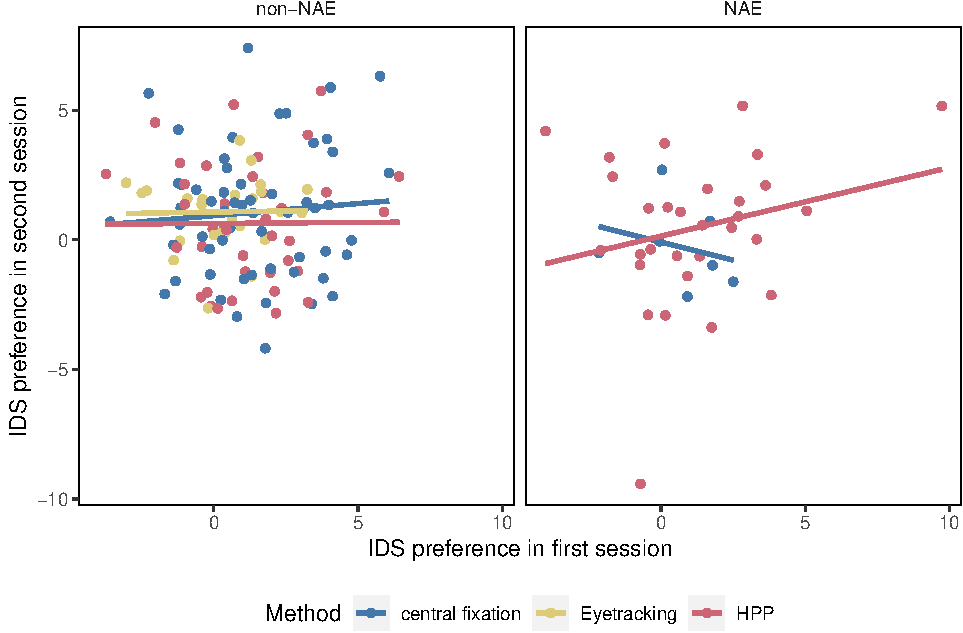
\includegraphics{MB1T_supplement_files/figure-latex/fig1-1.pdf}
\caption{\label{fig:fig1}Infants' preference in Session 1 and Session 2 with individual data points and regression lines color-coded by method (central fixation, eye-tracking, or HPP). Results are plotted separately for North American English-learning infants (right panel) and infants learning other languages and dialects (right panel).}
\end{figure}

NAE-learning infants showed greater IDS preferences than their non-NAE counterparts in MB1. We therefore also assessed if test-retest reliability interacted with children's language background. A multilevel analysis with Lab as random intercept, predicting the IDS preference in Session 2 based on the IDS preference in Session 1, NAE and the interaction of these two variables, revealed no interaction, \(\beta\)=0.29, \emph{SE}=0.18, \emph{p}=.115 (see Figure S1).

\hypertarget{s3-meta-analytic-estimate}{%
\subsection{S3: Meta-analytic estimate}\label{s3-meta-analytic-estimate}}

\hypertarget{s4-alternative-dependent-variables}{%
\subsection{S4: Alternative Dependent Variables}\label{s4-alternative-dependent-variables}}

\hypertarget{s4.1.-log-transformed-looking-times}{%
\subsubsection{S4.1. Log-transformed looking times}\label{s4.1.-log-transformed-looking-times}}

\hypertarget{s4.2.-proportion-novelty-preference.}{%
\subsubsection{S4.2. Proportion novelty preference.}\label{s4.2.-proportion-novelty-preference.}}

\hypertarget{s5-patterns-of-preference-across-sessions}{%
\subsection{S5: Patterns of preference across sessions}\label{s5-patterns-of-preference-across-sessions}}

We also conducted analyses to explore whether there were any patterns of preference reversal across test sessions.
While there was no strong correlation in the magnitude of IDS preference between test session 1 and test session 2, here we asked whether infants consistently expressed the same preference across test sessions.
Overall, 58.20\% of the infants had a consistent preference from test to retest session, indicating that infants were not more likely than chance to maintain their preference from test session 1 to test session 2 (exact binomial test; \emph{p} =
0.05).
Of the 158 total infants, 44.90\% of infants showed a consistent infant-directed speech preference and 13.30\% showed a consistent adult-directed speech preference.
23.40\% of infants switched from an infant-directed speech preference at test session 1 to an adult-directed speech preference at test session 2 and 18.40\% switched from an adult-directed speech preference to an infant-directed speech preference.

Next, we explored whether we could detect any systematic clustering of infants with distinct patterns of preference across the test and retest session.
We took a bottom-up approach and conducted a \emph{k}-means clustering of the test-retest difference data.
We found little evidence of distinct clusters emerging from these groupings: the clusterings ranging from \emph{k}=2 (2 clusters) to \emph{k}=4 (4 clusters) appear to simply track whether participants are approximately above or below the mean looking time difference for test session 1 and test session 2, and the diagnostic elbow plot shows little evidence of a qualitative improvement as the number of clusters is increased.

\begin{figure}
\centering
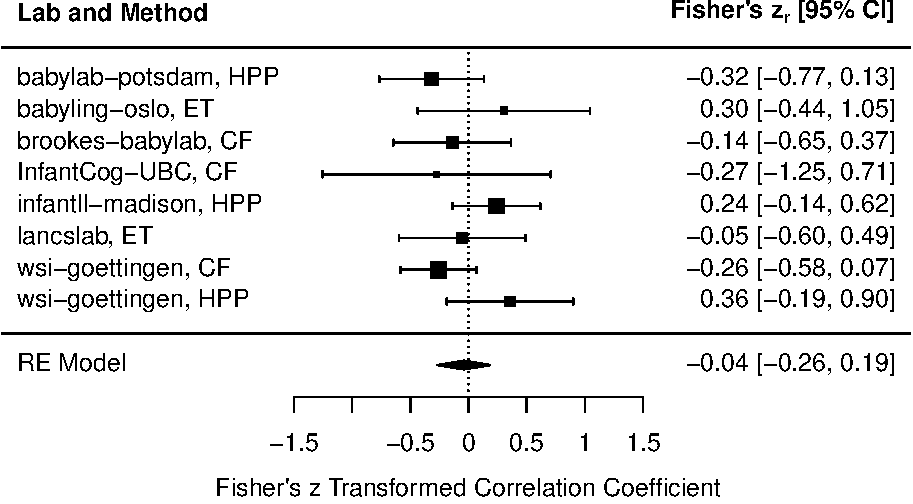
\includegraphics{MB1T_supplement_files/figure-latex/fig2-1.pdf}
\caption{\label{fig:fig2} (A) Results from the k-means clustering analysis of IDS preference in session 1 and 2 for different numbers of k and (B) the corresponding elbow plot of the total within-cluster sum of squares. In (A), points represent indvidual participants' magnitude of looking time difference at test sessions 1 (x-axis) and 2 (y-axis). The solid line indicates no preference for IDS vs.~ADS, the dotted lines indicate mean IDS preference at test session 1 and 2, respectively. Colors indicate clusters from the k-means clustering for different values of k.}
\end{figure}

\hypertarget{s6-relationship-between-the-number-of-trials-infants-contribute-in-each-session}{%
\subsection{S6: Relationship between the number of trials infants contribute in each session}\label{s6-relationship-between-the-number-of-trials-infants-contribute-in-each-session}}

\begin{figure}
\centering
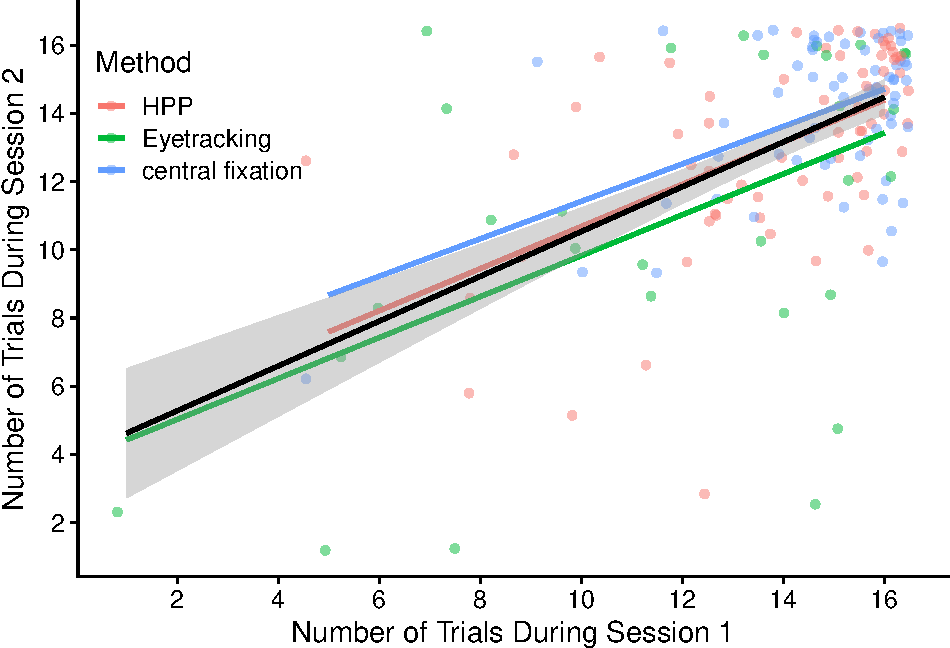
\includegraphics{MB1T_supplement_files/figure-latex/sfig1-1.pdf}
\caption{\label{fig:sfig1}Correlation between the number of trials contributed in session 1 and session 2. Each data point represents one infant. Colored lines represent linear fits for each method.}
\end{figure}

Are there stable individual differences in how likely an infant is to contribute a high number of trials?
To answer this question, we conducted an exploratory analysis investigating whether there is a relationship between the number of trials an infant contributed in session 1 and session 2.
Do infants who contribute a higher number of trials during their first testing session also tend to contribute more trials during their second testing session?
A positive correlation between trial numbers during the first and second session would indicate that their is some stability in a given infants' likelihood of remaining attentive throughout the experiment.
On the other hand, the absence of a correlation would indicate that the number of trials a given infant contributes is not predictive of how many trials they might contribute during their next session.

We found a strong positive correlation between number of trials contributed during the first and the second session \(r = .58\), 95\% CI \([.47, .68]\), \(t(159) = 9.05\), \(p < .001\) (see Figure 1).
This result suggests that if infants contribute a higher number of trials in one session, compared to other infants, they are likely to contribute a higher number of trials in their next session.
This finding is consistent with the hypothesis that how attentive infants are throughout an experiment (and hence how many trials they contribute) is a stable individual difference, at least for some infant looking time tasks.
Researchers should therefore be mindful of the fact that decisions about including or excluding infants based on trials contributed may selectively sample a specific sub-set of the infant population they are studying (Byers-Heinlein, Bergmann, \& Savalei, 2021; DeBolt, Rhemtulla, \& Oakes, 2020).

\hypertarget{s7-correlations-in-average-looking-times-between-sessions}{%
\subsection{S7: Correlations in average looking times between sessions}\label{s7-correlations-in-average-looking-times-between-sessions}}

\hypertarget{s7.1-relations-between-overall-looking-time-in-session-1-and-2.}{%
\subsubsection{S7.1: Relations between overall looking time in session 1 and 2.}\label{s7.1-relations-between-overall-looking-time-in-session-1-and-2.}}

There is a strong relationship between average overall looking in the first test session and the second test session, even after controlling for number of trials in the first and second session.

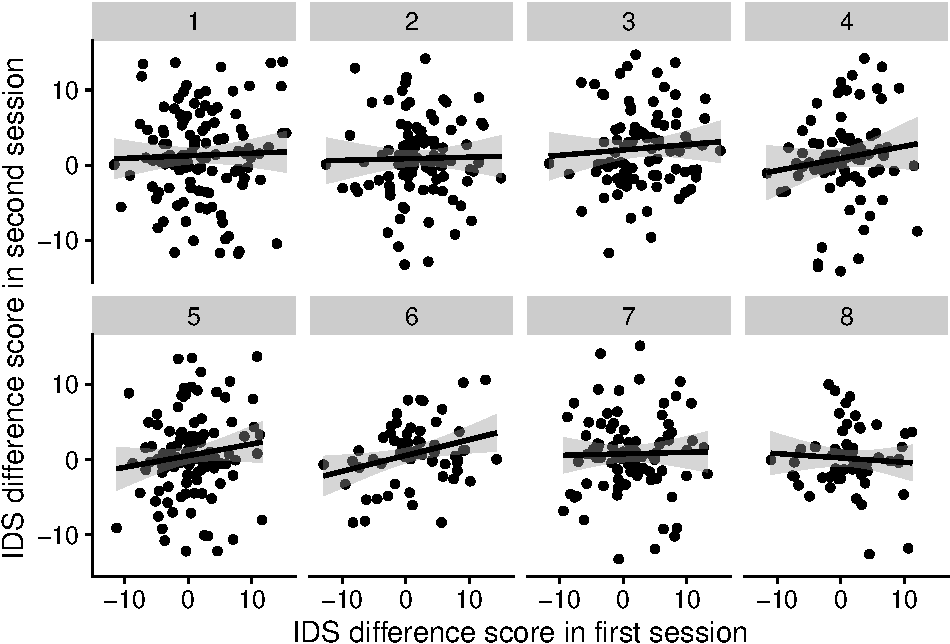
\includegraphics{MB1T_supplement_files/figure-latex/unnamed-chunk-8-1.pdf}

\begin{table}[tbp]

\begin{center}
\begin{threeparttable}

\caption{\label{tab:unnamed-chunk-8}Average Looking during session 1 predicted from average looking at session 2, controlling for trial number for each session.}

\begin{tabular}{llllll}
\toprule
Predictor & \multicolumn{1}{c}{$b$} & \multicolumn{1}{c}{95\% CI} & \multicolumn{1}{c}{$t$} & \multicolumn{1}{c}{$\mathit{df}$} & \multicolumn{1}{c}{$p$}\\
\midrule
Intercept & 2.55 & {}[0.38, 4.73] & 2.32 & 154 & .022\\
Mean lt 1 & 0.42 & {}[0.27, 0.58] & 5.52 & 154 & < .001\\
N 1 & -0.08 & {}[-0.24, 0.08] & -0.96 & 154 & .338\\
N 2 & 0.18 & {}[0.04, 0.32] & 2.52 & 154 & .013\\
\bottomrule
\end{tabular}

\end{threeparttable}
\end{center}

\end{table}

\hypertarget{s7.2-relations-in-overall-looking-time-to-ids-and-ads-stimuli.}{%
\subsubsection{S7.2: Relations in overall looking time to IDS and ADS stimuli.}\label{s7.2-relations-in-overall-looking-time-to-ids-and-ads-stimuli.}}

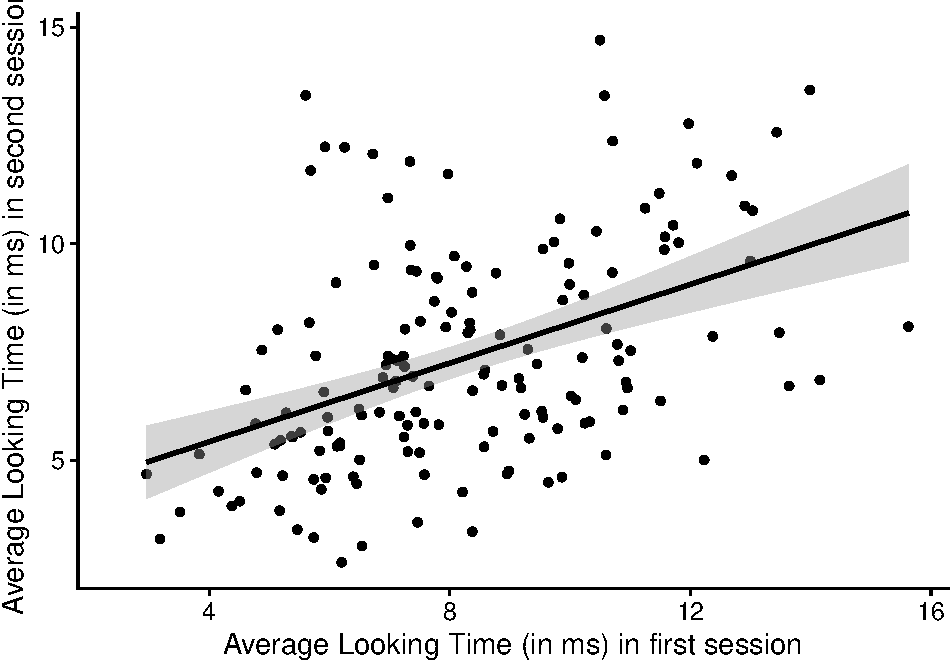
\includegraphics{MB1T_supplement_files/figure-latex/unnamed-chunk-9-1.pdf}

\begin{verbatim}
## 
## Call:
## lm(formula = LT_Retest_IDS ~ LT_Test_IDS + LT_Test_ADS, data = agg_by_subj_condition_paired_wide)
## 
## Residuals:
##     Min      1Q  Median      3Q     Max 
## -4.2721 -1.7567 -0.2799  1.4822  6.4805 
## 
## Coefficients:
##             Estimate Std. Error t value Pr(>|t|)    
## (Intercept)   3.9749     0.6902   5.759 4.41e-08 ***
## LT_Test_IDS   0.2123     0.1008   2.105   0.0369 *  
## LT_Test_ADS   0.2467     0.1044   2.362   0.0194 *  
## ---
## Signif. codes:  0 '***' 0.001 '**' 0.01 '*' 0.05 '.' 0.1 ' ' 1
## 
## Residual standard error: 2.52 on 155 degrees of freedom
##   (7 observations deleted due to missingness)
## Multiple R-squared:  0.1771, Adjusted R-squared:  0.1665 
## F-statistic: 16.68 on 2 and 155 DF,  p-value: 2.751e-07
\end{verbatim}

\begin{verbatim}
## 
## Call:
## lm(formula = LT_Retest_ADS ~ LT_Test_IDS + LT_Test_ADS, data = agg_by_subj_condition_paired_wide)
## 
## Residuals:
##    Min     1Q Median     3Q    Max 
## -5.556 -1.771 -0.489  1.254  8.901 
## 
## Coefficients:
##             Estimate Std. Error t value Pr(>|t|)    
## (Intercept)   3.2374     0.7356   4.401    2e-05 ***
## LT_Test_IDS   0.1103     0.1075   1.026  0.30641    
## LT_Test_ADS   0.3563     0.1113   3.201  0.00166 ** 
## ---
## Signif. codes:  0 '***' 0.001 '**' 0.01 '*' 0.05 '.' 0.1 ' ' 1
## 
## Residual standard error: 2.686 on 155 degrees of freedom
##   (7 observations deleted due to missingness)
## Multiple R-squared:  0.1677, Adjusted R-squared:  0.157 
## F-statistic: 15.62 on 2 and 155 DF,  p-value: 6.619e-07
\end{verbatim}

\hypertarget{s7.3-relations-for-specific-ads-and-ids-stimuli-between-the-first-and-second-session.}{%
\subsubsection{S7.3: Relations for specific ADS and IDS stimuli between the first and second session.}\label{s7.3-relations-for-specific-ads-and-ids-stimuli-between-the-first-and-second-session.}}

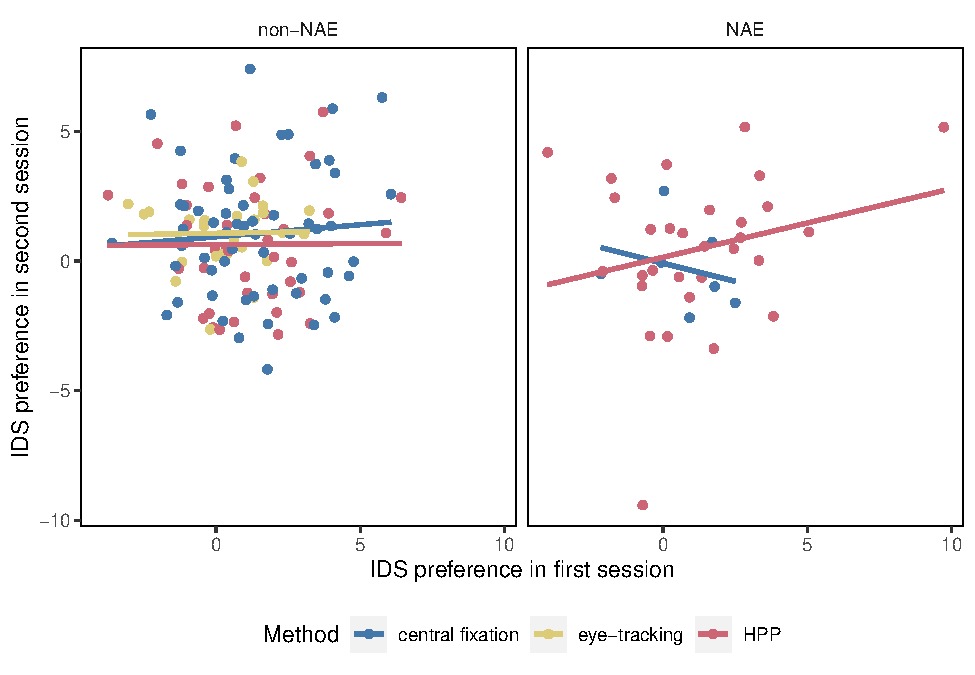
\includegraphics{MB1T_supplement_files/figure-latex/unnamed-chunk-11-1.pdf}

\begin{table}[tbp]

\begin{center}
\begin{threeparttable}

\caption{\label{tab:unnamed-chunk-11}Mixed-effects model results predicting looking time during session 1 from looking time at session 2 at the stimulus level.}

\begin{tabular}{llllll}
\toprule
Term & \multicolumn{1}{c}{$\hat{\beta}$} & \multicolumn{1}{c}{95\% CI} & \multicolumn{1}{c}{$t$} & \multicolumn{1}{c}{$\mathit{df}$} & \multicolumn{1}{c}{$p$}\\
\midrule
Intercept & 6.04 & {}[4.99, 7.08] & 11.35 & 6.88 & < .001\\
LT Test & 0.13 & {}[0.05, 0.20] & 3.46 & 25.38 & .002\\
\bottomrule
\end{tabular}

\end{threeparttable}
\end{center}

\end{table}

\hypertarget{s8-by-item-pair-preference-scores-across-sessions}{%
\subsection{S8: By-item-pair preference scores across sessions}\label{s8-by-item-pair-preference-scores-across-sessions}}

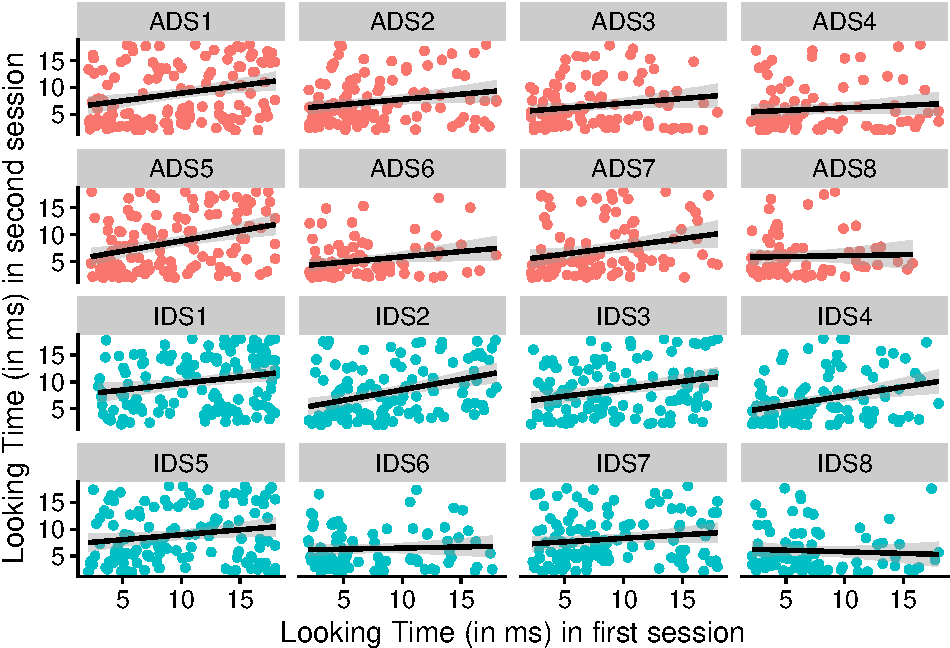
\includegraphics{MB1T_supplement_files/figure-latex/unnamed-chunk-12-1.pdf}

\begin{table}[tbp]

\begin{center}
\begin{threeparttable}

\caption{\label{tab:unnamed-chunk-12}Mixed-effects model results predicting IDS preference during session 1 from IDS preference at session 2 at the stimulus level.}

\begin{tabular}{llllll}
\toprule
Term & \multicolumn{1}{c}{$\hat{\beta}$} & \multicolumn{1}{c}{95\% CI} & \multicolumn{1}{c}{$t$} & \multicolumn{1}{c}{$\mathit{df}$} & \multicolumn{1}{c}{$p$}\\
\midrule
Intercept & 0.87 & {}[0.45, 1.30] & 4.04 & 122.79 & < .001\\
Diff 1 & 0.10 & {}[-0.02, 0.22] & 1.63 & 6.31 & .151\\
\bottomrule
\end{tabular}

\end{threeparttable}
\end{center}

\end{table}

\newpage

\hypertarget{references}{%
\section{References}\label{references}}

\begingroup
\setlength{\parindent}{-0.5in}
\setlength{\leftskip}{0.5in}

\hypertarget{refs}{}
\begin{CSLReferences}{1}{0}
\leavevmode\vadjust pre{\hypertarget{ref-byers2021six}{}}%
Byers-Heinlein, K., Bergmann, C., \& Savalei, V. (2021). Six solutions for more reliable infant research. \emph{Infant and Child Development}, e2296.

\leavevmode\vadjust pre{\hypertarget{ref-debolt2020robust}{}}%
DeBolt, M. C., Rhemtulla, M., \& Oakes, L. M. (2020). Robust data and power in infant research: A case study of the effect of number of infants and number of trials in visual preference procedures. \emph{Infancy}, \emph{25}(4), 393--419.

\leavevmode\vadjust pre{\hypertarget{ref-manybabies2020quantifying}{}}%
ManyBabies Consortium. (2020). Quantifying sources of variability in infancy research using the infant-directed-speech preference. \emph{Advances in Methods and Practices in Psychological Science}, \emph{3}(1), 24--52.

\end{CSLReferences}

\endgroup


\end{document}
